\section{AdaBoost (30 Points) (Xun)}

Consider $ m $ training examples $ S = \cbb{(x_1,y_1), \dotsc, (x_m, y_m)} $, where $ x \in \Xc$ and  $ y \in \cbb{-1, 1} $. 
Suppose we have a weak learning algorithm $ A $ which produces a hypothesis $ h: \Xc \to \cbb{-1,1} $ given any distribution $ D $ of examples. 
AdaBoost works as follows (slightly different from the lecture slides, but they are equivalent):
\begin{itemize}
\item 
Begin with a uniform distribution $ D_1(i) = \frac{1}{m} $, $ i = 1, \dotsc, m $.

\item 
At each round $ t = 1, \dots, T $,
\begin{itemize}
\item 
Run $ A $ on $ D_t $ and get $ h_t $. 

\item 
Update 
$ D_{t+1}(i) = \frac{D_t}{Z_t} e^{- \alpha_t y_i h_t(x_i)} $, 
where $ Z_t $ is the normalizer and $ i = 1, \dotsc, m $.
\end{itemize}

\end{itemize}

Note that since $ A $ is a weak learning algorithm, the produced $ h_t $ at round $ t $ is only slightly better than random guessing, say, by a margin $ \gamma_t $:
\begin{align}
\epsilon_t 
= \err_{D_t} (h_t) 
= \Pr\textstyle_{x \sim D_t} \sbb{y \ne h_t(x)}
= \frac{1}{2} - \gamma_t.
\end{align}

In the end, AdaBoost outputs $ H = \sgn \bb{\sum_{t=1}^{T} \alpha_t h_t} $ as the learned hypothesis. 
We will now prove that the training error $ \err_S(H) $ of AdaBoost decreases to zero at a very fast rate. 
In the answer, please state clearly why the derivation makes sense, for instance ``by Cauchy-Schwarz, ...''. 



\begin{enumerate}
\item 
Let's first justify the update rule. 
Imagine there is an adversarial who wants to fool $ h_t $ in the next round by adjusting the distribution. 
More formally, given $ h_t $, the adversarial wants to set $ D_{t+1} $ such that 
$ \err_{D_{t+1}} (h_t) = \half $. 
Show that the particular choice of $ \alpha_t = \half \log \frac{1-\epsilon_t}{\epsilon_t} $ achieves this goal. 

Note: why do we want such an adversarial setting? 
Because otherwise $ A $ might as well return $ h_t $ or $ -h_t $ again in round $ t+1 $ and still be slightly better than random guessing, which means it essentially learns nothing.


\item 
Show that 
$ D_{T+1}(i) = \bb{m \cdot \prod_{t=1}^{T} Z_t}\inv e^{- y_i f(x_i)} $, where $ f(x) = \sum_{t=1}^{T} \alpha_t h_t(x) $. 


\item\label{sec:bound1}
Show that $ \err_S(H) \le \prod_{t=1}^{T} Z_t $.


\item\label{sec:bound2} 
Show that $ \prod_{t=1}^{T} Z_t \le e^{-2\sum_{t=1}^{T} \gamma_t^2} $.

\item 
Now let $ \gamma = \min_t \gamma_t $. 
From \ref{sec:bound1} and \ref{sec:bound2}, we know the training error approaches zero at exponential rate with respect to $ T $. 
Then how many rounds are needed
to achieve a training error $ \varepsilon > 0 $? 
Please express in big-O notation, $ T = \Oc (\cdot) $.


 
\item 
Consider the data set in Figure~\ref{fig:toy}. 
Run $ T=3 $ iterations of AdaBoost with decision stumps (axis-aligned separators) as the base learners.
Illustrate the learned weak hypotheses $ \cbb{h_t} $ in Figure~\ref{fig:toy} and fill in Table~\ref{tbl:boost}. 
The MATLAB code that generates Figure~\ref{fig:toy} is available on the course website.

We recommend writing a simple program as it might be tedious to calculate by hand. 
It will also help you understand how it works in practice. 



\begin{table}[h]
\renewcommand{\arraystretch}{1.5}
\centering
\begin{tabular}{|c|c|c|c|c|c|c|c|c|c|c|c|c|}
\hline 
$ t $ 
& $ \epsilon_t $ 
& $ \alpha_t $ 
& $ D_t(1) $ 
& $ D_t(2) $ 
& $ D_t(3) $
& $ D_t(4) $
& $ D_t(5) $
& $ D_t(6) $
& $ D_t(7) $
& $ D_t(8) $
& $ D_t(9) $ 
& $ \err_S(H) $ \\
\hline 
1 & & & & & & & & & & & & \\
\hline 
2 & & & & & & & & & & & & \\
\hline 
3 & & & & & & & & & & & & \\
\hline 
\end{tabular}
\caption{AdaBoost results}
\label{tbl:boost}
\end{table}



\begin{figure}[t]
\centering
\subfigure{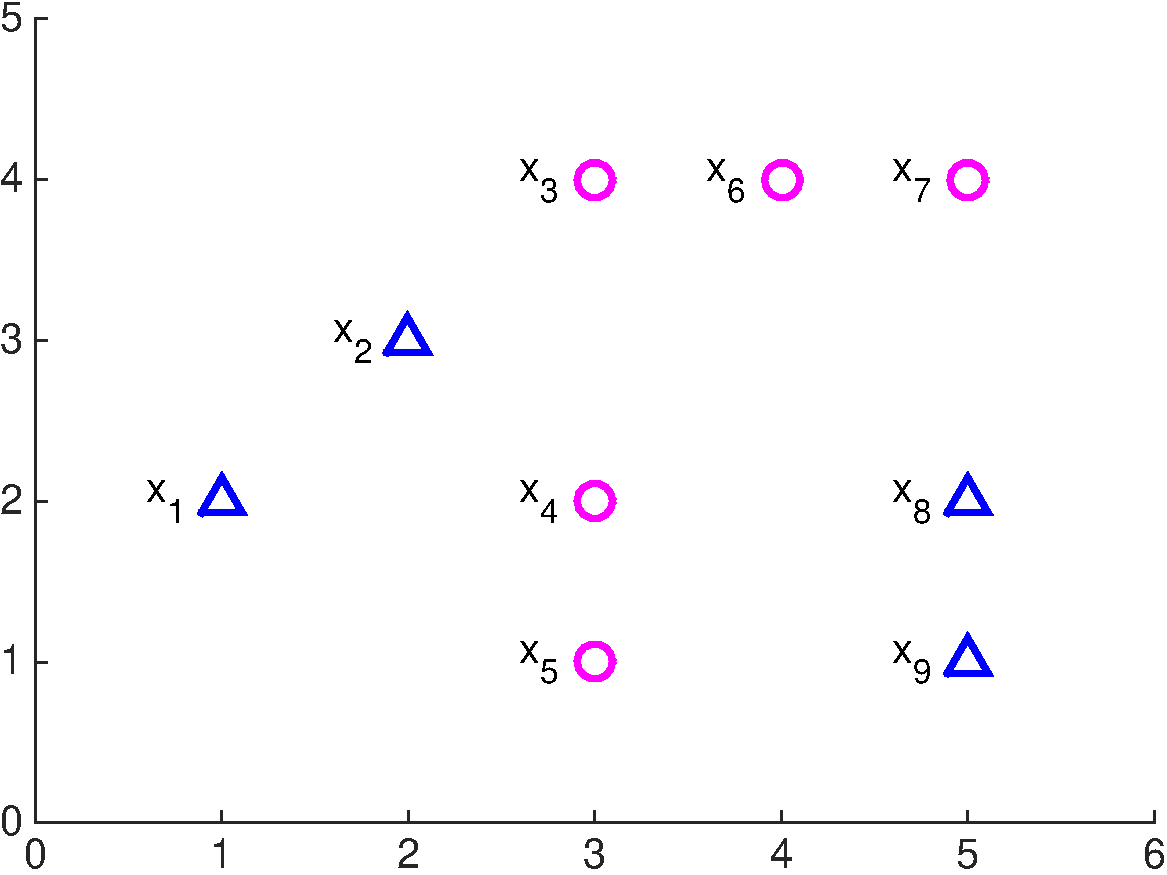
\includegraphics[width=.35\textwidth]{./adaboost.pdf}}
\caption{Toy data for AdaBoost.}
\label{fig:toy}
\end{figure}


\end{enumerate}